\section{Extreme value theory}
\label{sec:evt}
\subsection{Idealised statistical theory}
The central limit theorem is a well known triumph of classical statistics,
and it is often useful in the physical sciences where the central value
is that of interest. However, by its nature the mean SSH will
not be able to damage the coast (barring significant sea level rise that is not mitigated),
and life and property will only be put
at risk by the most extreme events.

The extreme value theorem is:


Let $X_{1}, X_{2} \ldots, X_{n} \ldots$ be a sequence of independent and
identically-distributed random variables, and $M_n = \max\{X_1, \ldots X_n\}$.
For a sequence of real numbers $(a_n, b_n) \exists: a_n>0$, and
$\lim _{n \rightarrow \infty} P\left(\frac{M_{n}-b_{n}}{a_{n}} \leq x\right)=F(x)$
where $F$ is a non-degenerate distribution function, then the limit distribution
$F$ belongs to either the Gumbel, the Frechet, or the Weibull family.
However as T19~\cite{taleb2019statistical} states, `life is lived in the pre-asymptotics',
and it is not clear how long it would take to converge.


Extreme value theory is the provides the extension of this theory
to look at the return period of extreme events of a certain value.

Both require domain of attraction condition~\cite{bucher2018horse}:

\begin{enumerate}
  \item Either $\forall r \in \mathbb{N} \;\exists \;b_r \in \mathbb{R},\; \gamma\in \mathbb{R},\; a_r>0: $
    \begin{eqnarray}
    \lim _{r \rightarrow \infty} F^{r}\left(a_{r} x+b_{r}\right)=\exp \left\{-(1+\gamma x)^{-1 / \gamma}\right\} \\
     \text { for all } 1+\gamma x>0
    \tag{BM}
    \end{eqnarray}

  \item Or equivalently, there exists a positive function $\psi=\psi (t):$
    \begin{eqnarray}
    \lim _{t \uparrow x^{*}} \frac{1-F(t+\psi(t) x)}{1-F(t)}=(1+\gamma x)^{-1 / \gamma} \\
    \text { for all } 1+\gamma x>0
    \tag{POT}
    \end{eqnarray}
 \end{enumerate}

Normal Choices are POT or Block Maxima, but these strategies require
large amounts of data to converge~\cite{taleb2019much}.

BM leads to Generalised Extreme Value (GEV) distribution,
      whereas POT leads to Generalised Pareto Distribution (GPD).

\subsection{Block maxima GEV}
It is trivial to extract the highest SSH value in a given year at a given point
from \texttt{control-1950}.
It was decided not to subtract the low frequency SSH seasonal cycle from the
values first, because it is the absolute height of the sea surface which
creates the hazard rather than the relative height.

\begin{figure*}[htb!]
    \centering
    \includegraphics[width=0.8\linewidth]{../surge/plots/GEV_modelNO.pdf}
    %\vspace{-25pt}
   \caption{New Orleans GEV plot for \texttt{control-1950} Interesting transition
            - does this represent hurricanes?}
    \label{fig:gev-no}
    \includegraphics[width=0.8\linewidth]{../surge/plots/skextreme_second_tactic.pdf}
    \vspace{-15pt}
   \caption{Confidence intervals not defined near Miami and Eastport. }
    \label{fig:gev_all_points}
\end{figure*}


\begin{figure*}[htb!]

\begin{minipage}{0.45\textwidth}

\includegraphics[width=1\linewidth]{../surge/plots/GEV_pi_plateau_NO.pdf}
\caption{First attempt at enforcing a GP asymptote of 2m for New Orleans,
with an \texttt{RBF} kernel.
The data is the same as in Figure~\ref{fig:gev-no}. The
kink is caused by using a non-differentiable mapping to
enforce the far-field conditions. 1$\sigma$ and 2$\sigma$ envelopes shown.}
\end{minipage}
\begin{minipage}{0.45\textwidth}

    \centering
    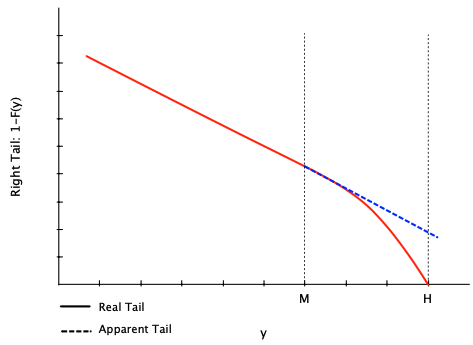
\includegraphics[width=1\linewidth]{images/taleb-limit-slimmed.png}\\
    \textit{Figure 15.1 from T19~\cite{taleb2019statistical} p.~279}
   \caption{As shown if you only
   observe a distribution up to some value M,
    you may be tempted to fit a line through the
   data (dotted blue line).
   But if there were in fact a limit to the distribution at H,
   you would be overestimating
   the true number of very extreme events (red curve),
   predicting events that were larger than were possible.}
   \label{fig:up-bound-taleb}
   \end{minipage}

   \begin{minipage}{0.45\textwidth}
   \centering
   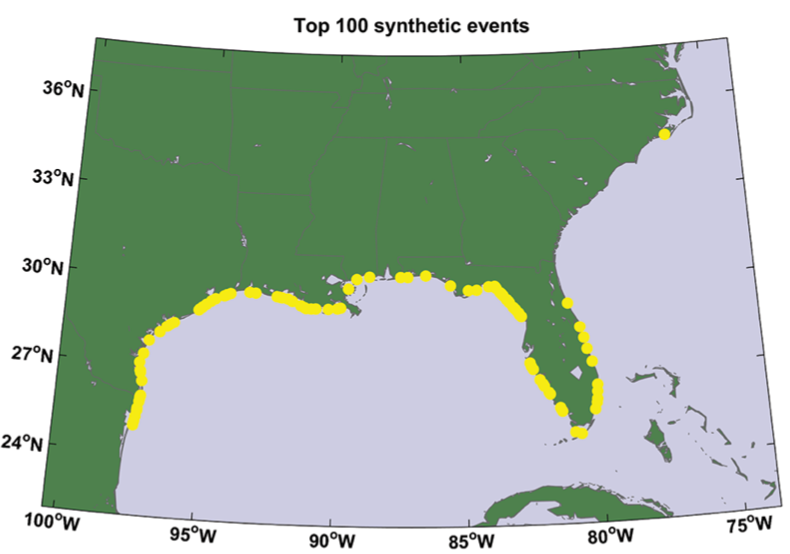
\includegraphics[width=1\linewidth]{images/top-100-landfalls.png}\\
   \textit{Figure 3b from \cite{emanuel2017will}}
   \caption{The top 100 most rapidly intensifying events in the model,
   showing that models capture far more of these TCs in the Gulf of Mexico
   and Florida than further north.
     }
   \label{fig:top-100}
   \end{minipage}
   \begin{minipage}{0.45\textwidth}
   \centering
   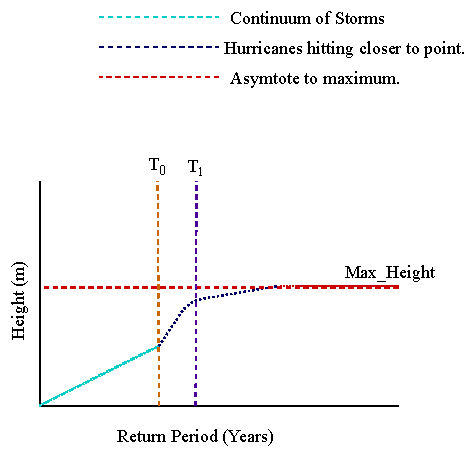
\includegraphics[width=1\linewidth]{images/Return_Hypothesis.pdf}
   \vspace{-15pt}
  \caption{The maximum height is a function of the potential intensity
  allowed by the climate, and the responsiveness of that point on the coastline to a
  wind stress of that size. If T$_0$, or T$_1$, is a similar or greater than the time period of
  measurement, then it is respectively possible that no hurricanes exist in the data sample,
  or that no hurricanes make direct landfall at that location.}
    \label{fig:return_hyp_new}
    \end{minipage}





\end{figure*}


\subsection{Comparison to POT GPD}
The other alternative is to use the peak-over-threshold method.
There are a number of alternatives as to how you should choose the
threshold.

\subsection{Enforcing an asymptote using potential intensity theory }
As noted in~§~\ref{sec:hurr-theory} there is some maximum size
that a tropical cyclone might be expected to be able to reach given
the climate. This gives us information as to the shape of the probability
distribution beyond what just curve-fitting the tail.


\begin{figure}[htb!]
    \centering
    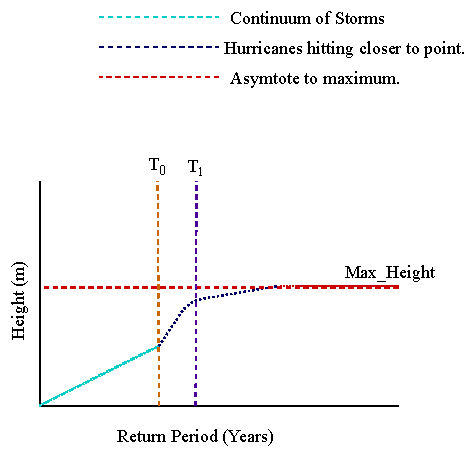
\includegraphics[width=1\linewidth]{images/Return_Hypothesis.pdf}
    \vspace{-15pt}
   \caption{The maximum height is a function of the potential intensity
   allowed by the climate, and the responsiveness of that point on the coastline to a
   wind stress of that size. If T$_0$, or T$_1$, is a similar or greater than the time period of
   measurement, then it is respectively possible that no hurricanes exist in the data sample,
   or that no hurricanes make direct landfall at that location.}
     \label{fig:return_hyp_new}

\end{figure}

